\documentclass{frontiersSCNS}

\usepackage{url,hyperref,lineno,microtype}
\usepackage[onehalfspacing]{setspace}
\linenumbers

%\usepackage[margin=1in,footskip=0.25in]{geometry}

%\usepackage{helvet}
%\renewcommand{\familydefault}{\sfdefault}

\renewcommand\refname{\vskip -1cm}


%\renewcommand{\rmdefault}{phv} % Arial
%\renewcommand{\sfdefault}{phv} % Arial
\usepackage{setspace}
\usepackage{wrapfig}
\usepackage{amsmath}
\usepackage{amssymb}
\usepackage{graphicx}
\usepackage{mathrsfs}
\usepackage{bm}
\usepackage{wasysym}
\usepackage{placeins}
\usepackage{multirow}
\usepackage[T1]{fontenc}
%\usepackage[super]{natbib}
\usepackage{framed}
\usepackage{caption}
\usepackage{longtable}


\def\keyFont{\fontsize{8}{11}\helveticabold }
\def\firstAuthorLast{Yeakel {et~al.}} %use et al only if is more than 1 author
\def\Authors{
Justin D. Yeakel\,$^{1,2,\dagger,*}$,
Uttam Bhat\,$^{1,\dagger}$,
Emma E. Smith\,$^3$,
and Seth D. Newsome\,$^3$}
% Affiliations should be keyed to the author's name with superscript numbers and be listed as follows: Laboratory, Institute, Department, Organization, City, State abbreviation (USA, Canada, Australia), and Country (without detailed address information such as city zip codes or street names).
% If one of the authors has a change of address, list the new address below the correspondence details using a superscript symbol and use the same symbol to indicate the author in the author list.
\def\Address{$^{1}$Santa Fe Institute, Santa Fe, New Mexico, USA \\
$^{2}$School of Natural Sciences, University of California, Merced, Merced, California, USA \\
$^{3}$Department of Biological Sciences, University of New Mexico, Albuquerque, New Mexico, USA \\
$^{\dagger}$Contributed equally}
% The Corresponding Author should be marked with an asterisk
% Provide the exact contact address (this time including street name and city zip code) and email of the corresponding author
\def\corrAuthor{Justin D. Yeakel}
\def\corrAddress{Santa Fe Instite, Santa Fe, New Mexico, 87505, USA}
\def\corrEmail{jdyeakel@gmail.com}


\begin{document}
\onecolumn
\firstpage{1}

\title[Exploring the isotopic niche]{Exploring the isotopic niche: isotopic variance, physiological incorporation, and the temporal dynamics of foraging}

\author[\firstAuthorLast ]{\Authors} %This field will be automatically populated
\address{} %This field will be automatically populated
\correspondance{} %This field will be automatically populated

\extraAuth{}% If there are more than 1 corresponding author, comment this line and uncomment the next one.
%\extraAuth{corresponding Author2 \\ Laboratory X2, Institute X2, Department X2, Organization X2, Street X2, City X2 , State XX2 (only USA, Canada and Australia), Zip Code2, X2 Country X2, email2@uni2.edu}


\maketitle


% \begin{document}
%
% \title{Isotopic incorporation and the temporal dynamics of foraging among individuals and within populations}
% \author{JD Yeakel, U Bhatt, SD Newsome}
% \maketitle

\begin{abstract}

%%% Leave the Abstract empty if your article falls under any of the following categories: Editorial Book Review, Commentary, Field Grand Challenge, Opinion or specialty Grand Challenge.
\section{}
%As a primary goal, the abstract should render the general significance and conceptual advance of the work clearly accessible to a broad readership. References should not be cited in the abstract.
For full guidelines regarding your manuscript please refer to \href{http://www.frontiersin.org/about/AuthorGuidelines}{Author Guidelines} \\ or \textbf{Table \ref{Tab:01}} for a summary according to article type.


\tiny
 \keyFont{ \section{Keywords:} Text Text Text Text Text Text Text Text } %All article types: you may provide up to 8 keywords; at least 5 are mandatory.
\end{abstract}


\section{Introduction}

Consumer foraging behaviors are dynamic, resulting in diets that change over time as a function of environmental conditions, the densities of consumer and resource populations, and even the physiological states of individual foragers.
Understanding how diets change, and to what extent different conditions promote or inhibit specific changes, is both a challenging theoretical and empirical problem in ecology.

Analysis of carbon and nitrogen stable isotopes of a consumer with respect to a suite of potential prey is a commonly used tool for determining diet.
As a consumer incorporates the isotopic values of its consumed resources into its tissues, it becomes a unique `blend' of its prey.
Determining the most likely proportional contribution of prey that determines a given consumer's diet has thus been the focus of intense interest (REFS).

Of additional interest are the factors that control the consumer's isotopic niche width, which is defined by the isotopic variance of the consumer at either the individual or population level.
A consumer's isotopic niche width, by definition, is a function of the isotopic values of its potential prey (the prey mixing space), as well as its dietary predilections.
For a given mixing space, a consumer with a large isotopic niche width may be incorporating many isotopically distinct prey into its diet, while a consumer with a small isotopic niche width may be specializing on a single resource.


%Difference between the isotopic diet view vs. other diet views

%Backward integrating vs. Forward integrating

%EXPLORE VARIANCE ~ what controls the isotopic niche?

%Prey-switching dynamic
%Micro time frame
%Macro time frame




\section{Methods \& Analysis}
We begin by establishing a forward-integration approach for modeling the incorporation of stable isotopes from multiple resources into a consumer's tissues.
This new methodology provides an analytical link between the mechanistic drivers of foraging and the distribution of stable isotope values that describes a consumer's tissues over time.
%This framework aims to provide a flexible platform for introducing additional ecological complexities, such as time-dependent foraging behaviors and dietary specialization both among and within individuals.
Using this framework, we aim to
1) examine how certain dietary behaviors, such as prey specialization and different modes of dietary variation, impact the isotopic variance of consumer tissues thus aiding ecological interpretation of the `isotopic niche', and
2) show how these methods can be expanded to include foraging behaviors that themselves are temporally dynamic, changing over seasons or years.

\subsection*{Deriving the within-individual isotopic niche width}
%The dynamics of diet ~ heuristic description of the process
There are many ways to statistically summarize the integration of prey by a consumer species, however in order to establish a mechanistic link between foraging and the consumer's isotopic distribution, we follow the proceeding heuristic foraging mechanic.

We assume that a consumer encounters and consumes resources in proportion to the encounter rate of each prey; prey that are encountered more frequently are assumed to be consumed more frequently.
An alternative approach could incorporate preferences (REFS) or even state-dependence (REFS), and we will briefly address these considerations in the Discussion.
As prey are encountered and consumed, the prey's isotope values are incorporated into the consumer's tissues weighted by the prey-specific proportional contribution to diet.
The resulting distribution that descibes the dietary input of multiple prey (each with an independent Gaussian density that describes the distribution of their isotopic values) is a mixed Gaussian distribution with weights determined by the prey's proportional contribution to diet.
This proportional contribution is itself a random variable drawn from a Dirichlet density (a multivariate Beta distribution) that serves as a probabilistic description of the consumer's dietary input.
The following section details our probabilistic description of the consumer dietary strategy, and focus our attention on the variability of the consumer isotopic distribution, which is equivalent to its isotopic niche width - a statistic of certain interest to ecologists using stable isotopes as a tool to understand diet.
%, as well as an analysis of the properties of the final consumer isotopic distribution.


%Derivation of the Dirichlet controlling diet
%If we  that the proportional contribution of prey to a consumer's diet scales to the rate at which it encounters its prey.
%, such that we must first describe how the Dirichlet distribution describing consumer diet at a given point in time changes as a function of prey densities.
A consumer encounters each prey at a frequency determined by a Poisson process with parameter $\lambda_i$, which determines the number of encounters $M_i(t)=m$ between time 0 and time $t$,

\begin{equation}
f_M (m_i|\lambda_i) = {\rm e}^{-\lambda_i t}\frac{(\lambda_i t)^m}{m!}.
\end{equation}

\noindent Here and henceforth, we use the general function $f(\cdot)$ to denote different frequency distributions, as well as uppercase notation to describe stochastic variables, and lowercase notation to describe specific values of stochastic variables.
If we assume that encounter rates are variable, such that some prey are more patchily distributed than others, we can treat $\Lambda_i = \lambda_i$ as a random variable with a Gamma density

\begin{equation}
f_\Lambda (\lambda_i | c, a_i) = \frac{c^{a_i}}{\Gamma (a_i)}{\rm e}^{-c \lambda_i}\lambda_i^{a_i - 1}.
\end{equation}

\noindent Here, $a_i$ is the dispersion parameter, and $c$ scales with the time between encounters.
If we integrate across all possible values of $\lambda_i$, we obtain the Negative Binomial density with mean encounter rate $a_i/c$ and coefficient of variation $1/\sqrt{a_i}$ (REF Mangel).
Following the derivation described by Ainsworth (REF), if we define the proportional contribution of prey to a consumer's diet to scale with the encounter rate, such that

\begin{equation}
  p_i = \frac{\lambda_i}{\sum_{j=1}^n \lambda_j},
\end{equation}

\noindent then the random variable $P_i \in {\bm P} = p_i \in {\bm p}$, where $\sum_i p_i = 1$, has a Dirichlet distribution with density

\begin{equation}
  f_{\bm P}(p_1,...,p_n|a_1,...,a_n) = \frac{\Gamma(\sum_{i=1}^n a_i)}{\sum_{i=1}^n\Gamma(a_i)}\prod_{i=1}^n p_i^{a_i - 1},
\end{equation}

\noindent where $\Gamma(\cdot)$ is the gamma function (REF Mangel).
We note that bold-face fonts denote vectors of variables.
As such, the expected proportional contribution of a prey $i$ to the consumer's diet has the expectation ${\rm E}\{p_i\}=a_i/a_0$ where $a_0 = \sum_i a_i$, and variance

\begin{equation}
  \label{eqDirVar}
  {\rm Var}\{p_i\} = \frac{a_i(a_0 - a_i)}{a_0^2(a_0 + 1)}.
\end{equation}

Describing the dietary behavior of a consumer as a Dirichlet distribution provides a flexible and powerful framework to investigate how different foraging strategies influence a consumer's isotopic niche.
For example, a pure generalist consumer would have a Dirchlet distribution with parameters $a_i = 1$ for all prey $i=1,...,n$, such that the marginal distribution for $P_i = p_i$ is close to uniform with expectation ${\rm E}\{p_i\} = 1/n$.
Because we have assumed that the proportional contribution of a prey to the consumer's diet scales with the prey's encounter rate, this would be analogous to a system where a consumer is equally likely to encounter the same number of any prey.
In contrast, an obligate specialist would have a Dirichlet density that is spiked for a given prey $k$, such that the single parameter $a_k \gg 1$, while $a_{i \neq k} = 1$.
The use of a Dirichlet distribution is also at the heart of Bayesian isotope mixing models (REFS), which assume a Dirichlet prior and enable the input of alternative dietary information to inform isotopic data.


%Describing Z
If the isotopic distributions for the set of potential prey follow independent Gaussian distributions, and the dietary behavior of the consumer has a Dirichlet density, the resultant density that describes the isotopic distribution of a consumer's diet $f_Z(Z=z)$ is a mixed Gaussian distribution, with weights given by ${\rm E}\{p_{i}\} = a_i/a_0$ for prey $i = 1,...,n$.
This density can be written as

\begin{equation}
f_Z(z|{\bm a},{\bm \mu},{\bm \sigma}) = \sum_{i=1}^n \frac{a_i}{a_0}\frac{1}{\sqrt{2 \pi \sigma_i^2}}{\rm e}^{-\frac{(z-\mu_i)^2}{2\sigma_i^2}},
\end{equation}

\noindent with the expectation

\begin{equation}
\label{eqEZ}
  {\rm E}\{Z\} = \sum_{i=1}^n \frac{a_i}{a_0} \mu_i,
\end{equation}

\noindent where $\mu_i$ is the mean isotopic value for prey $i$.
This is simply the weighted average of the isotopic values for the prey community, where weights are determined by the mean proportional contribution of prey to the consumer's diet.

Of more interest to us here is the variance of $f_Z(z)$, which will allow us to analytically determine the isotopic niche width of the consumer as a function of its dietary behavior and the isotopic distributions (or mixing space) of its prey.
We find that

\begin{equation}
\label{eqVarZ}
  {\rm Var}\{Z\} = \sum_{i=1}^n \frac{a_i}{a_0}\left(\sigma_i^2 + \mu_i^2\right) - \frac{a_i^2\mu_i^2}{a_0^2}-\sum_{i \neq j}\frac{a_i a_j \mu_i \mu_j}{a_0^2}.
\end{equation}

\noindent Although the form of Eq. \ref{eqVarZ} is not intuitive, we emphasize that - over different dietary behaviors that shape the Dirichlet distribution and for different isotopic mixing spaces - it is this equation that governs the expansion or contraction of the consumer's isotopic niche width, and therefore of chief ecological interest.

The isotopic variance of the consumer's diet ${\rm Var}\{Z\}$ can be simplified by considering a specific set of dietary behaviors.
Here we examine how ${\rm Var}\{Z\}$ is influenced by generalist vs. specialist consumer diets, as well as the role of general mixing space geometries, in determining consumer isotopic niche width.
If a generalist consumer alters its diet to become a specialist on a single prey, the Dirichlet distribution that defines its dietary behavior goes from $a_i=1$ for all $i=1,...,n$ to $a_{i \neq k}=1$ for $i=1,...,n$, with $a_k>1$.
As specialization increases, the Dirichlet parameter corresponding to the preferred prey $k$, increases to a value much higher than one (pure specialization is obtained only at the limit $a_k \to \infty$).
Thus, we can assume that $a_i=1$ for all $i \neq k$, and $a_k = (n-1)s_k/(1-s_k)$, where $s_k$ denotes specialization on prey $k$, ranging from $1/n$ (generalization) to $1$ (specialization).
We can thus substitute $a_0 = (n-1)/(1-s_k)$ and $p_i = a_i/a_0 = (1-s_k)/(n-1)$ for all $i \neq k$, and $a_k/a_0 = s_k$.
We can then rewrite Eq. \ref{eqVarZ} as

\begin{equation}
\label{eqVarZs}
{\rm Var}\{Z\} = \frac{1-s_k}{n-1}\sum_{i \neq k}^n \left(\sigma_i^2 + \mu_i^2\right) + s_k(\sigma_k^2 + \mu_k^2) - \left(\frac{1-s_k}{n-1}\sum_{i \neq k}^n \mu_i + s_k\mu_k \right)^2,
\end{equation}

\noindent and note that, independent of the prey mixing space (a function of $\mu_i$ and $\sigma_i^2$ for prey $i=1,...,n$), the isotopic variance of the consumer's diet will always be a concave parabolic function over $s_k$.
With respect to the size of the consumer's isotopic niche width, this means that there can be a peak variance for a value of $s_k$ intermediate to pure generalization ($s_k=1/n$) and pure specialization ($s_k=1$).

The peak, or inflection point $\hat s_k$, that describes the maximum isotopic variance of the consumer may or may not fall between $s_k=1/n$ and $s=1$, and is only of ecological interest if it does.
This inflection point can be solved analytically by setting the derivative of Eq. \ref{eqVarZs} with respect to $s_k$ equal to zero, and solving for $s_k$, which results in

\begin{equation}
	\hat s_k = \frac{A(1-n)+B (n-1)^2+2 C (C-D n+D)}{2 (C-D n+D)^2},
\end{equation}

\noindent where $A = \sum_{i \neq k}^n \left(\sigma_i^2 + \mu_i^2\right)$, $B = \left(\sigma_k^2 + \mu_k^2\right)$, $C = \sum_{i \neq k}^n \mu_i$, $D = \mu_k$.

Determination of the inflextion point for consumer isotopic variance allows us to predict where the consumer's isotopic niche is expected to be maximized as a function of specialization on different prey.
Although here we have focused on the special case where a consumer targets a single prey, one can rewrite the equation for the consumer's isotopic niche width with respect to increasing specialization on any number or combination of prey in the mixing space.
For example, in the case where a consumer specializes on two prey (i.e. two species of crab), one would rewrite Eq. \ref{eqVarZ} in terms of both $s_k$ (specialization on prey $k$) and $s_l$ (specialization on prey $l$), resulting in a concave parabolic sheet in dimensions $s_k$ and $s_l$.
Determining the maximum variance would then entail taking the derivative of Eq. \ref{eqVarZ} with respect to both $s_k$ and $s_l$.
In dimensions higher than 2, the process would be the same, with the goal of finding the maximum variance over a hyperplane with a number of dimensions determined by the number of prey on which the consumer is specializing.
Because specializing on multiple prey does not introduce anything conceptually unique, we consider only the case of a single-prey specialist.



\subsection*{The Dynamics of Isotopic Incorporation}
We have established a framework for analytically calculating the distribution of isotope values that characterizes a consumer's diet, composed of multiple, isotopically distinct prey.
The dietary behavior of the consumer is a function of a single Dirichlet distribution, which is assumed not to change over time, although we will relax this assumption later on.
Due to the central limit theorem, over long timescales the dietary distribution of the consumer is static, with a fixed mean and variance.
However, over short timescales, the diet of the consumer varies as Eq. \ref{eqDirVar}, while its isotopic values vary by the combined effects of the Dirichlet and the mixed Gaussian framework, shown in Eq. \ref{eqVarZ}.

As the consumer incorporates prey into its diet, the dietary isotopic distribution is incorporated into its tissues.
The timescale of physiological isotopic incorporation is based on the turnover rate of consumer tissues, which on the fast end can occur within days to weeks (blood plasma), and on the slow end occur over years (bone).
Incorporation rates are well known to isotope ecologists and have been observed in both controlled feeding studies (REFS), and occasionally in the wild (REFS?).
Although the physiological details are not well understood, isotopic incorporation can be modeled using either single- or multi-compartmental approaches (REFS).
In a single compartment framework, isotope ratios are ingested with food, and directly incorporated into consumer tissues at a tissue-specific rate.
In multiple compartment frameworks, it is assumed that incorporation occurs over multiple body pools, the turnover of each occuring at different rates.
Though an assumption of multi-compartmental incorporation often does provide better statistical fit with experimental data, the physiological processes that drive incorporation of isotope ratios from one compartment to the other are not well understood, and such fits are only marginally better than a single-compartment approach.

In this next section, we assume the ingested isotope ratios are incorporated into consumer body tissues directly, moderated by the rate of incorporation $\lambda$, which is treated as a free parameter.
Thus, we aim to determine the isotopic compostion of the consumer $X_c$ as a function of the consumer diet, the isotopic distribution of its prey (or mixing space), and $\lambda$.
% The carbon and nitrogen isotope composition of a consumer's tissues are a product of its diet.
% If this diet incorporates multiple prey in different quantities, as is the case for most consumers, the resulting consumer isotopic distribution must take into account:
% \emph{i}) the initial isotopic signature of the consumer's tissues at a point in time $X_c(t)$ (we will assume for simplicity that the isotopic value in question is the ratio of heavy to light carbon isotope relative to a known standard $\delta^{13}{\rm C}$, though are methods are equivalent for any isotope that is integrated through diet),
% \emph{ii}) the isotopic values of $n$ resources, which we assume are Gaussian distributed with expectation $\mu_i$ and variance $\sigma_i^2$,
% %$\sum_{i=1}^n p_i \mu_i$ (where $p_i$ is the proportional contribution of resource $i$ and $\mu_i$ is the mean isotopic value of resource $i$),
% \emph{iii}) the rate at which each prey species is ingested by the consumer, summarized by its proportional contribution $p_i$,
% and
% \emph{iv}) the incorporation rate of a consumer's diet into its tissue $\lambda$.
In a completely deterministic framework, the isotopic composition of the consumer can be written as an ordinary differential equation

\begin{equation}
\label{eqODE}
\dot X_c = (1-\lambda)X_c + \lambda \sum_{i=1}^N p_i \mu_i - X_c
\end{equation}

\noindent where the overdot denotes the derivative with respect to time $t$, and $p_i$ and $\mu_i$ are the proportional contribution of prey $i$ to the diet of the consumer, and the mean isotopic value of prey $i$, respectively.

However, we must also take into account the stochastic effects described in the previous section, and here we consider two indepedent sources of variation.
First, each potential resource $i$ is composed of individuals with isotopic values varying according to independent Gaussian distributions with expecation ${\rm E}\{X_i\}=\mu_i$, and variance ${\rm Var}\{X_i\}=\sigma^2_i$.
Secondly, in this section we consider a consumer diet is variable, yet static (such that it can be described by a time-invariant probability distribution), there is variation in the consumption of prey across short periods of time.
% In other words, a consumer's diet is described by a probability distribution that itself is temporally static (a constraint that we will ease later on).

%Integration over time with a static diet
%{\bf The Dynamics of Incorporation.}
% The isotopic distribution of a consumer changes with the consumption of different prey.
% The extent of this change is a function of
% 1) the difference between the isotopic value of the consumer compared to its diet, and
% 2) the incorporation rate.
% Because the consumer's diet is stochastic, we must take into account both the isotopic expectation of diet, as well as the isotopic variance of diet, and this will allow us to determine both the expectation and variance of the consumer's isotopic value as a give dietary isotopic distribution is incorporated over time.

The consumer's isotopic distribution changes in accordance to the stochastic differential equation

\begin{equation}
\label{eqSDE}
{\rm d}X_c = (1-\lambda)X_c{\rm dt} + \lambda\left({\rm E}\{Z\}{\rm dt} + \sqrt{{\rm Var}\{Z\}}{\rm dW}\right) - X_c{\rm dt}.
\end{equation}

\noindent where ${\rm dW}$ is the increment of Brownian motion (REF MANGEL).
This stochastic differential equation is generally known as an Orstein-Uhlenbeck process (more?).
Because the time interval is infinitely short at the continuous time limit, the consumer's isotopic distribution will have a Gaussian density.
In this case, if the initial isotopic values of the consumer at time $t=0$ is $X_c(0)$, the expectation and variability of $X_c$ at time $t$ are

\begin{align}
{\rm E}\{X_c(t)\} &= {\rm E}\{Z\} + (X_c(0) - {\rm E}\{Z\}){\rm e}^{-\lambda t}, \nonumber \\
{\rm Var}\{X_c(t)\} &= \frac{\lambda {\rm Var}\{Z\}}{2}\left(1 - {\rm e}^{-2\lambda t}\right).
\end{align}

\noindent where ${\rm E}\{Z\}$ and ${\rm Var}\{Z\}$ are as defined in Eqns. \ref{eqEZ} and \ref{eqVarZ}.
One can observe that as $t$ increases, the exponential part of ${\rm E}\{X_c(t)\}$ and ${\rm Var}\{X_c(t)\}$ go to zero, such that ${\rm E}\{X_c(t)\} \to {\rm E}\{Z\}$, and ${\rm Var}\{X_c(t)\} \to \lambda{\rm Var}\{Z\}/2$.
In other words, the expectation of the consumer's isotopic distribution will equilibrate to that of its diet, while its variance will always be less than the variance of its diet by a factor of $\lambda/2$.
This decrease in variance is due to the fact that the consumer-diet mix has a biased weight towards its own body tissues, such that $\lambda < 1(2)$. %if \lamabda = 2, then it will look like what it eats... weird... worth going into at all?




% This is in accordance with known exponentially-decaying isotopic values of consumers shown in controlled-diet experiments (REFS).

%By uniting both dietary and isotopic variability into the single random variable $Z$, the above framework provides a means towards predicting the isotopic composition of a consumer over time, given a dietary strategy (described by the Dirichlet distribution) and the isotopic distribution of the potential resources (the isotopic mixing space).
%Permitting the consumer's dietary strategy to vary provides a direct means of incorporating behavioral variability in estimates of a consumer's isotopic composition.




\section{Results}

As a consumer samples from multiple prey with stable isotopes values following independent Gaussian distributions, its tissues become a mixture of these distributions.
The weights that control the contributions of each prey to the consumer mix are determined by the dietary behavior of the consumer, which we have shown follows a Dirichlet distribution.
The use of the Dirichlet distribution in this context follows previous ecological models by Ref(Ainsworth, others?), and is also used as a prior in Bayesian isotope mixing models.
We note that Bayesian mixing models are essentially models that explore the opposite question that we are investigating: they are used to estimate the dietary behavior of the consumer (the posterior probability distribution for the proportional contribution vector $\bm p$) given the isotopic distributions of both consumer and prey, whereas we are investigating factors that impact the isotopic distribution of the consumer as a function of different prey mixing spaces and consumer dietary behaviors.


We have provided an analytical solution for the mean and variance of the consumer's isotope distribution as a function of its diet and the isotope mixing space.
By formulating these solutions in terms of consumer generalization and specialization, we consider three important observations:
1) the variance of the consumer's isotope distribution (${\rm Var}\{Z\}$), which is equivalent to its isotopic niche width, is concave parabolic;
2) whether and to what extent the ${\rm Var}\{Z\}$ demonstrates measurable nonlinearity depends in part on the geometry of the mixing space;
3) the inversion point, or the peak, of ${\rm Var}\{Z\}$ over the generalization-specialization continuum is the consumer's maximum isotopic niche width.
This point may or may not exist at a value intermediate to an obligate generalist or obligate specialist.


%1-2: Concave parabolic variance curve & geometry of mixing space
The width, or variance, of the consumer's isotopic niche is necessarily concave parabolic over the specialization metric $s$, where $s=1/n$ refers to an obligate generalist, and $s=1$ refers to an obligate specialist.
This means that there is a peak isotopic variance that lies somewhere along this specialization continuum, however it is only of interest to us of it lies in $s \in [1/n,1]$.


One can gain some intuitive understanding of this nonlinearity by considering the following example, illustrated in Fig. \ref{figvar}.
In a 3-prey system, where all prey have equal isotope means and variance, a consumer that ranges from generalizing on all three prey to specializing on a single prey will have equivalent dietary isotope distributions.
As the mean value for the isotopic distribution of the targeted prey is moved away from the others, such that its offset from the centroid is increased, the variance function displays nonlinearity.
This can be understood by considering two prey with the same mean value, and the targeted prey with a very different mean value.
As the consumer incorporates isotopic ratios from all three prey in equal proportions, it will have increased isotopic variance due to the large spread of the prey.
As the consumer integrates this isotopically atypical prey in greater proportions, the heterogeneity of incorporated isotope ratios will increase, serving to increase its own isotopic variability.
The isotopic variability will then decline as it begins specializing on the atypical prey, and if it is consuming this prey exclusively, the isotopic variability of its diet will reflect the isotopic variability of its prey exactly.
The concave parabolic nature of consumer isotopic variability can thus be explained by heterogeneous incorporation of isotope ratios over an asymmetric mixing space.



%3: Inversion point location
Understanding what dietary strategy or mixing space geometry can maximize the isotopic niche width of the consumer will serve to help ecologists determine what mechanisms - ecological or statistical - may be driving isotopic data.
Our analytical solution for this inflection over dietary specialization ($\hat s$) reveals that maximum isotopic niche width can, but doesn't always, fall in $s \in [1/n,1]$.
If the peak lies outside of this region, changes in isotopic variance as specialization on a targeted prey is increased will appear monotonic or even linear.

Although the specific nature of $\hat s$ will depend strongly on mixing space geometry, we can determine certain key ingredients that will determine the general nature of where this value falls.
For mixing space geometries where the targeted prey has higher than average variance, $\hat s$ will tend to lie towards specialization, however the offset of the mean value for the targeted prey from the mixing space centroid will push $\hat s$ towards $s=0.5$ (Fig. \ref{figspecvar}A,B).
In contrast, if the targeted prey has lower than average variance, $\hat s$ will tend to lie towards generalization (Fig. \ref{figspecvar}B,C).
As before, if the offset of the targeted prey's mean value increases, $\hat s \to 0.5$.
In both cases, if the mean value for the targeted prey is close to the mixing space centroid, the maximum isotopic variance for the consumer could lie anywhere.

%Otter example

%Incorporation results

%%Static results (primary)
\emph{
\begin{itemize}
  \item Consumer isotopic niche width is concave parabolic
  \item This means that there is a maximum isotopic niche width for the consumer; this maximum value may lie between the consumer being a generalist or a specialist
  \item {\bf see figure 2:} Where the maximum value lies is a function of the mixing space...
  \begin{itemize}
    \item If the targeted prey has a higher than average variance, the maximum variance for the consumer will tend to be on the specialist side of the specialization metrix
    \item If the targeted prey has a lower than average variance, the maximum variance for the consumer will tend to be on the generalist side of the spectrum
  \end{itemize}
  \item Where the maximum value lies also has to do with how different the targeted prey's mean value is from the rest of the isotope mixing space (the offset).
  \begin{itemize}
    \item If the offset is low (such that the targeted prey's mean is near... but not on... the centroid), the maximum consumer niche width can be very close to the `generalization' or `specialization' side of the spectrum.
    \item If the offset is HIGH (such that the targeted prey's mean is far from the centroid), the maximum consumer niche width becomes very close to $s=0.5$...
  \end{itemize}
  \item {\bf see Figure 3:} This is not theoretical... we see that the consumer isotopic variance shows these properties for different targeted prey in the sea otter example!
\end{itemize}
}

%The variance is concave parabolic

%When does it peak for specialisits?
%When does it peak for generalists?
%Real world example (sea otters)

%Diet -> tissue: variability is scaled by lambda/2


%%Dynamic results



\section{Discussion}


%Static

%Introducing preferences and/or state dependence thought



\subsection{Temporal dietary dynamics}
An implicit assumption of the static model is that the consumer's diet varies instantaneously over a given parameterization of $f_Z(Z)$.
This will be relevant for organisms that have a consistently varying diet over time, however most organisms have diets that undergo large shifts over time, such that the Dirichlet distribution that might characterize their diets during one temporal window might be different the the Dirichlet distribution that characterizes their diet in another window in time.
Such a shift might be due to seasonal, ontogenetic, or demographic changes in the consumer's prey base.
In the following section, we will relax the assumption that diet is characterized by a single Dirichlet distribution over time, thus generalizing the dietary/isotopic dynamics as a function of time.

We now assume that diet (but not the isotopic distribution of prey) changes over time, such that the random variable of interest is now $Z(t)$.
Solving for $X(t)$, we find

\begin{align}
{\rm E}\{X(t)\} = X(0){\rm e}^{-\lambda t} + \lambda{\rm e}^{-\lambda t} \int_{s=0}^t {\rm e}^{\lambda s} {\rm E}\{Z(s)\}{\rm d}s, \nonumber \\
{\rm Var}\{X(t)\} = \lambda^2 {\rm e}^{-2\lambda t} \int_{s=0}^t {\rm e}^{2\lambda s} {\rm Var}\{Z(s)\} {\rm d}s
\end{align}

\noindent where $Z(t)$ is the time trajectory of the consumer diet's isotopic values.
Because we have assumed that the isotopic distributions of resources are constant, only the dietary strategy of the consumer can change through time.
For example, we might assume that if the consumer prefers prey 1 over prey 2 in the first part of the year, and prey 2 over prey 1 in the second part of the year, the expectation of the proportional contribution of prey to the diet of the consumer might oscillate sinusoidally over a year.
Because the isotopic values of prey are incorporated into the tissues of the consumer non-instantaneously, we would expect that the isotopic realization of such a dietary shift to be offset in time from the actual shift in prey.

Incorporating different classes of prey-switching dynamics permits an understanding of how the isotopic composition of a consumer reflects changes in its behavior over time as a function of the incorporation rate $\lambda$.
To gain an intuitive understanding of how ecological dynamics are portrayed by consumer isotope values, we consider two types of prey-switching behavior: {\it i}) an instantaneous shift from one dietary strategy to another (such as those used in feeding experiments), and {\it ii}) a sinusoidally varying dietary strategy.


%Linking our approach to population dynamics


%Final statement


\begin{figure}[h!]
\centering
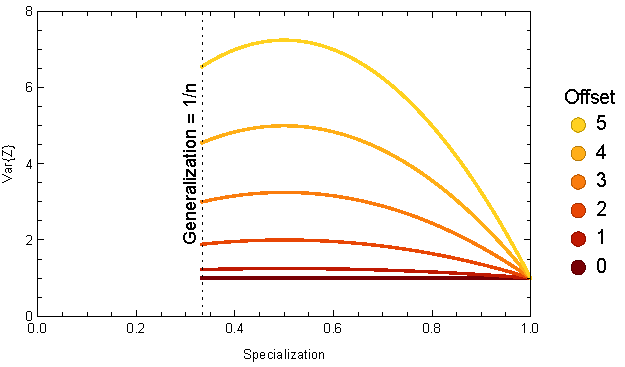
\includegraphics[width=0.5\textwidth]{fig_var.pdf}
\caption{
Variance of the isotopic distribution of diet with respect to specialization on a single prey, ${\rm Var}\{Z(s)\}$.
This illustrative example shows a three-prey system with prey means $\{-15,-15+\mbox{offset},-15\}$ and equal variances; colors depect specialization on prey 2 with a mean isotopic value that is a function of some offset amount.
As the offset of the targeted prey increases, so does the nonlinear nature of ${\rm Var}\{Z\}$.
}
  \label{figvar}
\end{figure}

\begin{figure}[h!]
\centering
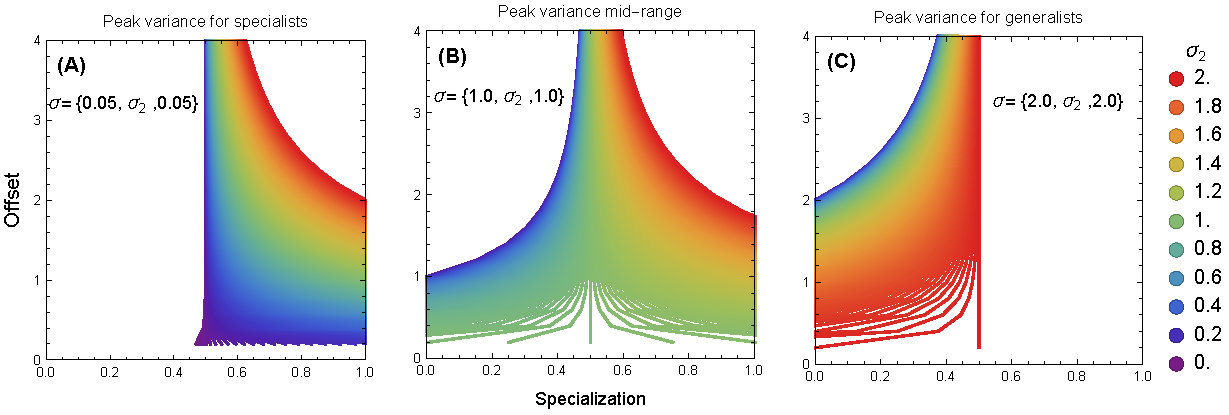
\includegraphics[width=1\textwidth]{fig_specvar.pdf}
\caption{
Maximal consumer isotopic varaince (niche width) over the specialization index $s$ as a function of mixing space geometry. A specialization value of $s=1/n$ denotes obligate generalization, while $s=1$ denotes obligate specialization.
Left, center, and right panel show the effect of different mixing space geometries on the location of maximal consumer niche width over $s$.
All panels: as the mean offset of the targeted prey is farther from the centroid of the mixing space, the maximal consumer isotopic niche width tends towards $s=0.5$.
Left and Center panel: If the targeted prey has a higher than average isotopic variance, the maximum consumer niche width will lie towards consumer specialization.
Center and Right panel: If the targeted prey has a lower than average isotopic variance, the maximum consumer niche width will like towards consumer generalization.
}
  \label{figspecvar}
\end{figure}



\begin{figure}[h!]
\centering
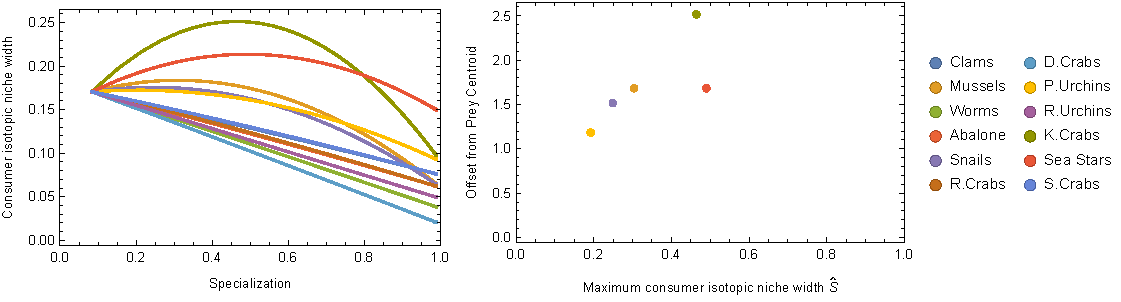
\includegraphics[width=1\textwidth]{fig_ottervar.pdf}
\caption{
Left panel: Predicted sea otter isotopic niche width over different degrees of specialization on each prey in the system (colors).
Right panel: Calculated maximum consumer niche width values as a function of specialization and the offset of the prey mean from the mixing space centroid.
}
  \label{figottervar}
\end{figure}


\end{document}
